\documentclass[11pt,a4paper]{article}
\usepackage[T1]{fontenc}
\usepackage{lmodern}
\usepackage{geometry}
\geometry{margin=23mm}
\usepackage{microtype}
\usepackage{amsmath,amssymb}
\usepackage{booktabs,longtable,array,tabularx}
\usepackage{enumitem}
\usepackage{xcolor}
\usepackage{listings}
\usepackage{tikz}
\usetikzlibrary{arrows.meta,positioning,shapes.geometric,calc,fit}
\usepackage{hyperref}
\usepackage{fancyhdr}
\usepackage{caption}
\usepackage{float}
\usepackage{parskip}

\definecolor{codebg}{RGB}{247,248,250}
\definecolor{codeframe}{RGB}{210,214,220}
\definecolor{commentgreen}{RGB}{0,105,68}
\definecolor{keywordblue}{RGB}{25,70,155}
\definecolor{stringred}{RGB}{150,35,35}

\lstdefinestyle{cstyle}{
  language=C,
  basicstyle=\ttfamily\small,
  keywordstyle=\color{keywordblue}\bfseries,
  commentstyle=\color{commentgreen}\itshape,
  stringstyle=\color{stringred},
  backgroundcolor=\color{codebg},
  frame=single,
  rulecolor=\color{codeframe},
  numbers=left,
  numberstyle=\tiny\color{gray},
  numbersep=8pt,
  showstringspaces=false,
  tabsize=4,
  breaklines=true,
  columns=fullflexible,
  keepspaces=true,
  captionpos=b
}

\setlist[itemize]{topsep=3pt,itemsep=2pt}
\setlist[enumerate]{topsep=3pt,itemsep=3pt}
\setlength{\headheight}{14pt}
\setlength{\parindent}{0pt}
\emergencystretch=2em

\pagestyle{fancy}
\fancyhf{}
\lhead{SmartSafe Project}
\rhead{4 x 4 Keypad Module}
\cfoot{\thepage}

\hypersetup{
  colorlinks=true,
  linkcolor=blue!60!black,
  urlcolor=blue!60!black,
  pdftitle={SmartSafe 4x4 Keypad Module},
  pdfauthor={Microprocessors End-Term Project}
}

\title{\textbf{SmartSafe Master Unit}\\[4pt]
\Large Complete Design and Code Explanation of the 4 x 4 Matrix Keypad Module}
\author{Microprocessors End-Term Project}
\date{July 2026}

\begin{document}
\maketitle
\thispagestyle{empty}

\begin{abstract}
This report documents the 4 x 4 matrix-keypad subsystem used by the SmartSafe Master. It explains the physical row-column switch matrix, the mixed-port pin assignment chosen to avoid conflicts with SPI, USART, Timer1, ADC, and the analog comparator, the ATmega32 data-direction, output, and input registers, the reason columns use internal pull-up resistors, the reason one row is driven low at a time, the complete scanning sequence, the relationship between physical coordinates and the software key map, input settling time, edge-style key reporting, limitations of the present debounce method, ghosting and simultaneous-key behavior, and integration with the password-entry state machine. The module does not require a dedicated timer or communication baud rate; those absences are also explained rather than hidden.
\end{abstract}

\tableofcontents
\newpage

\section{Purpose of the Keypad}
The keypad is the local user-input device of the SmartSafe Master. It provides ten decimal digits and several function keys. The application accepts only:
\begin{itemize}
  \item digits \texttt{0} through \texttt{9}, which are stored in a four-character password buffer;
  \item \texttt{C}, which clears the current partial password.
\end{itemize}
After four digits are entered, the main loop automatically checks the password. The \texttt{E}, arithmetic, decimal-point, and division keys are ignored by the password logic.

\section{How a 4 x 4 Matrix Keypad Is Constructed}
A 4 x 4 keypad contains 16 normally open switches arranged at the intersections of four row conductors and four column conductors. Pressing a key electrically connects exactly one row to exactly one column.

\begin{figure}[H]
\centering
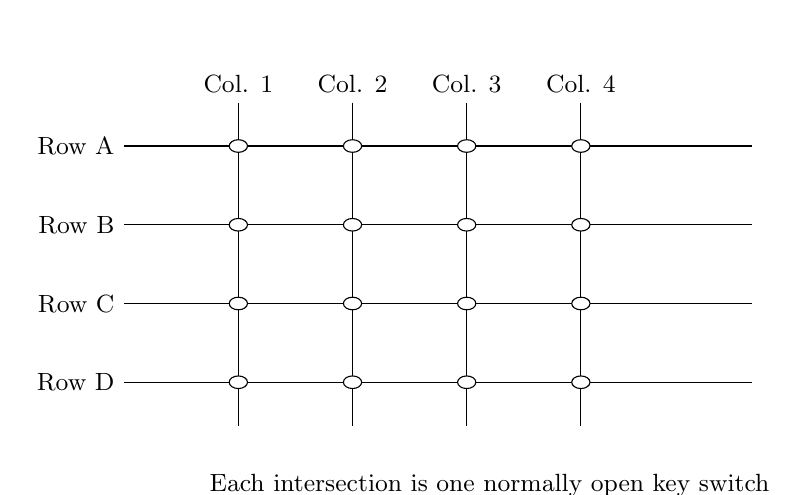
\begin{tikzpicture}[x=1.45cm,y=1.0cm,>=Latex,every node/.style={font=\small}]
\foreach \r/\label in {0/A,1/B,2/C,3/D}{
  \draw (-0.4,-\r) -- (5.1,-\r);
  \node[left] at (-0.4,-\r) {Row \label};
}
\foreach \c/\label in {0/1,1/2,2/3,3/4}{
  \draw (\c+0.6,0.55) -- (\c+0.6,-3.55);
  \node[above] at (\c+0.6,0.55) {Col. \label};
}
\foreach \r in {0,1,2,3}{
  \foreach \c in {0,1,2,3}{
    \draw[fill=white] (\c+0.6,-\r) circle (0.08);
  }
}
\node[below=5mm] at (2.8,-3.55) {Each intersection is one normally open key switch};
\end{tikzpicture}
\caption{Electrical organization of the matrix keypad.}
\end{figure}

Only eight microcontroller pins are required for sixteen keys. A separate input pin for every key would require sixteen pins.

\section{Final SmartSafe Pin Assignment}
The final mapping avoids all peripheral conflicts:
\begin{center}
\begin{tabular}{lll}
\toprule
Keypad terminal & ATmega32 pin & Direction during scanning \\
\midrule
A & PA4 & Output row 0 \\
B & PA5 & Output row 1 \\
C & PA6 & Output row 2 \\
D & PA7 & Output row 3 \\
1 & PD3 & Input column 0 with pull-up \\
2 & PD4 & Input column 1 with pull-up \\
3 & PB0 & Input column 2 with pull-up \\
4 & PB1 & Input column 3 with pull-up \\
\bottomrule
\end{tabular}
\end{center}

This mixed-port arrangement is deliberate:
\begin{itemize}
  \item PB4--PB7 are reserved for the hardware SPI EEPROM;
  \item PB3 is the AIN1 power-monitor input;
  \item PD0 and PD1 are USART RXD and TXD;
  \item PD2 is the INT0 wake button;
  \item PD5 is OC1A for the servo;
  \item PA3 is ADC3 for the tamper potentiometer;
  \item PA0 and PA2 control the LCD.
\end{itemize}

\section{Physical Key Layout and Key Map}
For the final Proteus calculator keypad, the intended mapping is:
\begin{center}
\begin{tabular}{c|cccc}
\toprule
 & Column 1 & Column 2 & Column 3 & Column 4 \\
\midrule
Row A & 7 & 8 & 9 & / \\
Row B & 4 & 5 & 6 & * \\
Row C & 1 & 2 & 3 & - \\
Row D & C & 0 & E & + \\
\bottomrule
\end{tabular}
\end{center}
The matching C array is:
\begin{lstlisting}[style=cstyle,caption={Key map matching the final Proteus component layout.}]
static const char keymap[4][4] = {
    { '7', '8', '9', '/' },
    { '4', '5', '6', '*' },
    { '1', '2', '3', '-' },
    { 'C', '0', 'E', '+' }
};
\end{lstlisting}
The key map is not an arbitrary software choice. Its row and column indices must correspond to the actual labels and terminal order of the selected Proteus component.

\section{ATmega32 GPIO Register Model}
Every port uses three important registers:
\begin{center}
\begin{tabular}{lll}
\toprule
Register & When written/read & Meaning \\
\midrule
\texttt{DDRx} & Written & Select input (0) or output (1) for each pin \\
\texttt{PORTx} & Written & Output level for output pins; pull-up control for input pins \\
\texttt{PINx} & Read & Actual logic level currently present at the pin \\
\bottomrule
\end{tabular}
\end{center}

For a column input with an internal pull-up:
\begin{lstlisting}[style=cstyle]
DDRx  &= ~(1U << bit);  /* input */
PORTx |=  (1U << bit);  /* internal pull-up enabled */
\end{lstlisting}
For an output row driven HIGH:
\begin{lstlisting}[style=cstyle]
DDRx  |= (1U << bit);
PORTx |= (1U << bit);
\end{lstlisting}
For the selected output row driven LOW:
\begin{lstlisting}[style=cstyle]
DDRx  |=  (1U << bit);
PORTx &= ~(1U << bit);
\end{lstlisting}

\section{Why Columns Use Internal Pull-Ups}
When no key is pressed, a keypad column is otherwise disconnected. A disconnected CMOS input is floating and may read either HIGH or LOW because of noise, leakage, or simulation state. The internal pull-up resistor gives every idle column a defined HIGH state without four external resistors.

\begin{figure}[H]
\centering
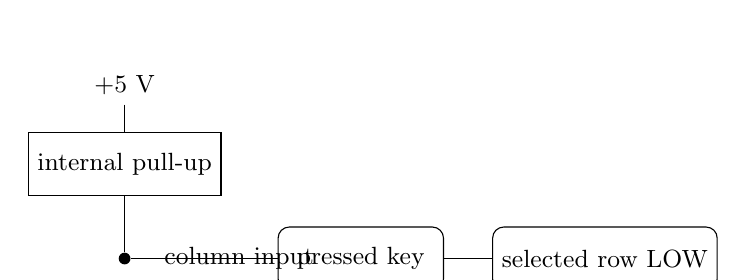
\begin{tikzpicture}[>=Latex,every node/.style={font=\small}]
\node (vcc) at (0,2.2) {+5 V};
\node[draw,minimum width=15mm,minimum height=8mm] (r) at (0,1.2) {internal pull-up};
\node[circle,fill=black,inner sep=1.5pt] (col) at (0,0) {};
\node[right=3mm of col] {column input};
\node[draw,rounded corners,minimum width=21mm,minimum height=8mm] (key) at (3.0,0) {pressed key};
\node[draw,rounded corners,minimum width=25mm,minimum height=8mm] (row) at (6.1,0) {selected row LOW};
\draw (vcc) -- (r) -- (col);
\draw (col) -- (key) -- (row);
\end{tikzpicture}
\caption{A pressed key overcomes the weak pull-up and connects the selected column to the LOW row.}
\end{figure}

With no key pressed, the column reads HIGH. With a key pressed on the currently selected row, it reads LOW.

\section{Why One Row Is Pulled LOW at a Time}
The selected row must drive the opposite level from the column idle bias. Since the columns idle HIGH through pull-ups, the active row is LOW. Pressing a key then changes the corresponding column from HIGH to LOW.

Rows are selected one at a time because the software must identify both coordinates. If every row were LOW simultaneously, a LOW column would identify the column but not which of the four keys in that column was pressed.

The reverse electrical method is possible: columns could use external pull-down resistors and one row could be driven HIGH. The ATmega32 provides internal pull-ups but no internal pull-downs, so active-LOW row scanning uses fewer components.

\section{GPIO Abstraction Used by the Driver}
Because the rows and columns are spread across PORTA, PORTB, and PORTD, the driver stores register addresses and bit numbers in a small structure:
\begin{lstlisting}[style=cstyle]
typedef struct {
    volatile uint8_t *ddr;
    volatile uint8_t *port;
    volatile uint8_t *pin;
    uint8_t bit;
} gpio_t;
\end{lstlisting}
Arrays then describe the eight keypad terminals. The same helper routines can configure a pin regardless of which AVR port owns it. This is cleaner than duplicating separate register expressions for each row and column.

\section{Complete Scanning Sequence}
A non-blocking scan follows this sequence:
\begin{enumerate}
  \item configure all four rows as HIGH outputs;
  \item configure all four columns as pull-up inputs;
  \item for row 0 through row 3:
  \begin{enumerate}[label=\alph*.]
    \item return every row HIGH;
    \item drive the current row LOW;
    \item wait briefly for the electrical levels to settle;
    \item read all four column inputs;
    \item when a column is LOW, convert the row-column pair through the key map;
  \end{enumerate}
  \item return every row HIGH;
  \item report a newly pressed key once.
\end{enumerate}

\begin{lstlisting}[style=cstyle,caption={Core matrix scan.}]
for (uint8_t r = 0; r < 4U; r++) {
    for (uint8_t rr = 0; rr < 4U; rr++)
        gpio_output_high(&rows[rr]);

    gpio_output_low(&rows[r]);
    __asm__ volatile ("nop\n\tnop\n\tnop\n\tnop\n\t");

    for (uint8_t c = 0; c < 4U; c++) {
        if (gpio_is_low(&cols[c])) {
            pressed = keymap[r][c];
            break;
        }
    }

    if (pressed)
        break;
}
\end{lstlisting}

\section{Settling Delay Calculation}
The driver uses four \texttt{NOP} instructions after changing the active row. Each \texttt{NOP} consumes one CPU clock cycle. At 8 MHz:
\[
T_{CPU}=\frac{1}{8\,000\,000}=0.125\ \mu\text{s}.
\]
Four instructions therefore provide approximately
\[
4\times0.125=0.5\ \mu\text{s}
\]
of explicit delay, in addition to the execution time of surrounding instructions. A keypad matrix has very small capacitance and low operating speed, so this is adequate for the Proteus simulation and ordinary short wiring.

No timer register is required for this settling delay. Using a hardware timer for a fraction of a microsecond would add configuration overhead larger than the intended delay.

\section{Key Detection Logic}
The helper reads the actual input register:
\begin{lstlisting}[style=cstyle]
static uint8_t gpio_is_low(const gpio_t *g)
{
    return ((*(g->pin) & (1U << g->bit)) == 0U);
}
\end{lstlisting}
The driver must read \texttt{PINx}, not \texttt{PORTx}. \texttt{PORTx} holds the output latch or pull-up setting; it does not necessarily represent the external electrical level.

\section{One Report per Press}
The driver uses a static state variable:
\begin{lstlisting}[style=cstyle]
static char last_reported = 0;
\end{lstlisting}
The behavior is:
\begin{itemize}
  \item no key currently detected: clear \texttt{last\_reported};
  \item same key remains held: return zero;
  \item different or newly pressed key: return that character and remember it.
\end{itemize}
This prevents one long press from filling all four password positions in successive main-loop iterations.

\section{Debounce: What the Present Code Does and Does Not Do}
The edge-style state suppresses repeated reports while the key remains continuously detected. It is not a complete time-based debounce algorithm. A mechanical contact can briefly alternate between pressed and released during the first several milliseconds. If one scan sees no key and the next scan sees the key again, \texttt{last\_reported} may be cleared and the same physical press could theoretically be reported twice.

Proteus keys are usually clean enough for the current approach. A physical design can add a timer-based confirmation, for example requiring the same row-column result for 20 ms before acceptance. The existing Timer2 compare interval is approximately 9.984 ms, so two or three stable Timer2 intervals can provide approximately 20--30 ms of debounce without a blocking delay.

\section{Why the Keypad Module Has No Baud Rate}
Baud rate is a serial-communication concept. The keypad is directly connected to GPIO pins and does not transmit asynchronous serial frames. Therefore:
\begin{itemize}
  \item no USART register is configured by the keypad driver;
  \item no baud-rate calculation applies to the keypad itself;
  \item the CPU clock matters only for scan execution time and the short NOP settling interval.
\end{itemize}
The Master later uses USART to report the result of password processing, but that communication belongs to the application and USART modules rather than the keypad electrical interface.

\section{Integration with the Main Loop}
The main loop calls:
\begin{lstlisting}[style=cstyle]
char key = keypad_scan();
if (!key)
    continue;
\end{lstlisting}
A valid key resets the inactivity counter. The application then handles it as follows:
\begin{itemize}
  \item \texttt{C}: clear the buffer and redraw the prompt;
  \item \texttt{0}--\texttt{9}: display an asterisk and append the digit;
  \item every other key: ignore it;
  \item four digits: compare the buffer with the password stored in internal EEPROM.
\end{itemize}
The keypad is intentionally ignored during lockout, while the servo is open, and during event-related UI holds. This policy is enforced by the main loop rather than the low-level keypad driver.

\section{Simultaneous Keys, Ghosting, and Output Contention}
A simple matrix without a diode at every switch is designed primarily for one key at a time. Multiple keys can create ambiguous current paths known as ghosting. Some combinations can also connect a HIGH nonselected row to the LOW selected row through two closed keys.

For a four-digit safe password, the user is expected to press and release one key at a time, so the simple matrix is adequate. A production keyboard requiring reliable multi-key operation would use per-key diodes or a dedicated keypad controller.

\section{Register and Constant Summary}
\begin{longtable}{p{0.24\textwidth}p{0.28\textwidth}p{0.40\textwidth}}
\toprule
Item & Selection & Reason \\
\midrule
\endhead
\texttt{DDRA4--7} & outputs & Four keypad rows. \\
\texttt{PORTA4--7} & one LOW at a time & Select one active row against HIGH-biased columns. \\
\texttt{DDRD3, DDRD4, DDRB0, DDRB1} & inputs & Four keypad columns. \\
Corresponding \texttt{PORT} bits & 1 while inputs & Enable internal pull-ups. \\
Corresponding \texttt{PIN} bits & read & Observe actual column levels. \\
\texttt{F\_CPU} & 8 MHz & System clock; gives 0.125 microsecond per CPU cycle. \\
NOP count & 4 & About 0.5 microsecond explicit settling time. \\
Rows/columns & 4 and 4 & Sixteen keys using eight MCU pins. \\
Dedicated timer & none & Scanning is quick and non-blocking; no periodic timer is required. \\
Baud rate & not applicable & The keypad is a direct GPIO matrix, not a serial device. \\
\bottomrule
\end{longtable}

\section{Proteus Test Procedure}
\begin{enumerate}
  \item Set the ATmega32 clock property to 8 MHz.
  \item Verify terminals A--D connect to PA4--PA7.
  \item Verify terminals 1--4 connect to PD3, PD4, PB0, and PB1.
  \item Start the simulation and confirm the Master LCD shows \texttt{Enter Password:}.
  \item Press one digit. Exactly one asterisk should appear.
  \item Hold the key. Additional asterisks should not appear.
  \item Release and press the same key again. A second asterisk should appear.
  \item Press \texttt{C}; all partial input should be cleared.
  \item Enter four digits and verify automatic password processing.
\end{enumerate}

\section{Common Failure Modes}
\begin{longtable}{p{0.31\textwidth}p{0.61\textwidth}}
\toprule
Symptom & Likely cause and correction \\
\midrule
\endhead
Every key returns the wrong symbol & Key-map rows or columns do not match the Proteus terminal order. \\
No key is detected & Rows/columns are wired incorrectly, column pull-ups are disabled, or the Master is in sleep/lockout/hold state. \\
One press enters several digits & Edge state was removed or switch bounce requires timed debounce. \\
A column always reads LOW & Short circuit, a key is held, or the selected pin direction is wrong. \\
SPI EEPROM stops working & Keypad was connected to PB4--PB7, conflicting with hardware SPI. \\
C key does not clear input & Physical C key is at a different row-column location than the software key map. \\
\bottomrule
\end{longtable}

\section{Conclusion}
The keypad module converts a 16-key switch matrix into a unique row-column coordinate by driving one row LOW at a time and reading four pull-up columns. The design uses the ATmega32 internal pull-ups, so no external column resistors are required. Mixed-port GPIO descriptors avoid conflicts with the project peripherals, four NOP instructions provide a short settling interval, and the static last-key state prevents repeated entry while a key is held. No USART baud rate or dedicated timer is required because the keypad is a directly scanned GPIO device.

\begin{thebibliography}{9}
\bibitem{atmega}
Microchip Technology Inc., \emph{ATmega32A Data Sheet}, sections on I/O ports, internal pull-ups, and instruction timing.\\
\href{https://ww1.microchip.com/downloads/en/DeviceDoc/Atmega32A-Data-Sheet-DS40002072A.pdf}{Official Microchip PDF}

\bibitem{project}
Microprocessors End-Term Project, \emph{Smart Safe with Remote Alarm}, project specification supplied with the implementation.

\bibitem{source}
SmartSafe source files: \texttt{keypad.c}, \texttt{keypad.h}, \texttt{config.h}, and \texttt{main.c}, July 2026 project version.
\end{thebibliography}

\end{document}
